\documentclass[10pt,a4paper]{article}
\usepackage[margin=2.2cm]{geometry}
\usepackage{graphicx}
\usepackage{booktabs}
\usepackage{siunitx}
\usepackage{amsmath}
\usepackage{float}
\usepackage{caption}
\usepackage{verbatim}
\usepackage{tikz}
\usetikzlibrary{arrows.meta, positioning, calc}
\usepackage[hidelinks]{hyperref}
\sisetup{detect-all}
\setlength{\emergencystretch}{2em}

\input{results.tex}

\IfFileExists{meas.tex}{\title{ASICONE ring oscillators: measurement and simulation}}{\title{ASICONE ring oscillators: expected results}}
\author{RISCVConsole bench, ULX3S + IHP130 QFN48 adapter}
\date{\today\\[2pt]\small Simulation data set: \texttt{\ResultsDir}}

\begin{document}
\maketitle

\section*{Summary}
\IfFileExists{meas.tex}{The measurement on the bench and its comparison with the post-layout simulation are in
Sections~\ref{sec:meas} and~\ref{sec:cmp}. }{}The first sections give the results expected \emph{before} the measurement, from transistor-level simulation of
the two ring oscillators of ASICONE (typical corner, \SI{1.2}{V}, \SI{27}{\celsius}). The bench reads
the output pads, which carry the ring divided by 32, with a counter in the FPGA over a \SI{1}{s} window.
\begin{center}
\begin{tabular}{lcc}
\toprule
 & RO13 & RO101 \\
\midrule
Ring frequency, TT & \SI{\RingA}{MHz} & \SI{\RingB}{MHz} \\
Ring frequency, all corners & \SIrange{\RingMinA}{\RingMaxA}{MHz} & \SIrange{\RingMinB}{\RingMaxB}{MHz} \\
Output pad (ring / 32), TT & \SI{\PadA}{MHz} & \SI{\PadB}{MHz} \\
Counts in \SI{1}{s} (\texttt{ro\_test}), TT & \CountA & \CountB \\
Stage delay, TT & \SI{\StageA}{ps} & \SI{\StageB}{ps} \\
Ring supply current, TT & \SI{\CurA}{mA} on RO2VDD & \SI{\CurB}{mA} on ROVDD \\
Supply sensitivity near \SI{1.2}{V} & \SI{\VddSensA}{\percent} per \SI{100}{mV} & \SI{\VddSensB}{\percent} per \SI{100}{mV} \\
Temperature coefficient & \SI{\TempSensA}{\percent/\celsius} & \SI{\TempSensB}{\percent/\celsius} \\
\bottomrule
\end{tabular}
\end{center}
The ratio $f_{13}/f_{101}$ is \RatioAB{} at TT and stays within \RatioMin--\RatioMax{} over the five
corners. Measuring both rings on the same chip therefore gives a check that does not depend on the
process corner.

\section{The circuit}
Each RO (\texttt{ro\_reliability}, cells \texttt{top\_13} and \texttt{top\_101}) is a ring of 13 or 101
inverting stages followed by a 5-flop ripple divider (\texttt{div\_sg13g2\_stdcells}, $\div 32$, reset by
\texttt{RO\_RST\_B}, active low) that drives a \SI{16}{mA} output pad. All stages are \texttt{lv} MOS with
$L = \SI{0.45}{\micro m}$, $W_p/W_n = 4 \times \SI{3.4}{\micro m} / 4 \times \SI{1.3}{\micro m}$. Three
stages are special:
\begin{itemize}
  \item \texttt{rovcel3}: inverter with header and footer driven by \texttt{n\_RO\_control} and
        \texttt{RO\_control}; it closes or opens the ring. When the ring is open, a transmission gate
        connects its output (the DUT input) to the \texttt{DUT\_gate} pin.
  \item \texttt{rovcel1}, the device under test: inverter with a PMOS header (gate \texttt{DUT\_Header},
        on when 0) and an NMOS footer (gate \texttt{DUT\_Footer}, on when 1). Its output is the
        \texttt{extra\_load} node, wired directly to an analog pad, and, when the ring is open, to
        \texttt{Drain\_Force}/\texttt{Drain\_Sense} through transmission gates.
  \item \texttt{rovcel4}: inverter with a PMOS header driven by \texttt{n\_RO\_control}.
\end{itemize}

\begin{figure}[H]\centering
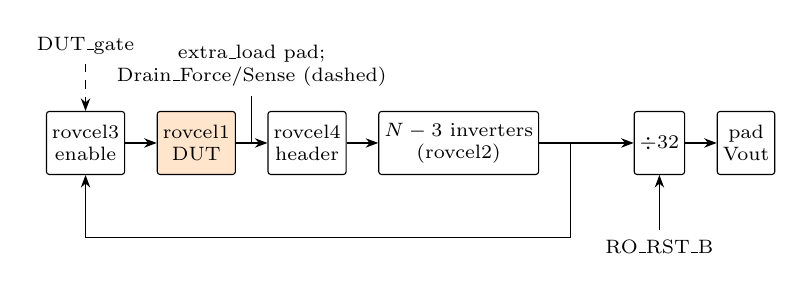
\begin{tikzpicture}[font=\scriptsize, node distance=4mm,
  blk/.style={draw, rounded corners=1pt, minimum height=8mm, align=center, inner sep=2pt},
  >={Stealth[length=1.6mm]}]
  \node[blk] (c3) {rovcel3\\enable};
  \node[blk, right=of c3, fill=orange!20] (c1) {rovcel1\\DUT};
  \node[blk, right=of c1] (c4) {rovcel4\\header};
  \node[blk, right=of c4] (inv) {$N-3$ inverters\\(rovcel2)};
  \node[blk, right=12mm of inv] (div) {$\div 32$};
  \node[blk, right=of div] (pad) {pad\\Vout};
  \draw[->] (c3) -- (c1);
  \draw[->] (c1) -- node[pos=0.45, below=5mm, align=center] (ex) {} (c4);
  \draw[->] (c4) -- (inv);
  \draw[->] (inv) -- (div);
  \draw[->] (div) -- (pad);
  \draw[->] ($(inv.east)+(4mm,0)$) -- ++(0,-12mm) -| (c3.south);
  \node[above=6mm of c3] (dg) {DUT\_gate};
  \draw[->, dashed] (dg) -- (c3.north);
  \coordinate (n1) at ($(c1.east)!0.5!(c4.west)$);
  \node[above=6mm of n1, align=center] (exl) {extra\_load pad;\\Drain\_Force/Sense (dashed)};
  \draw[-] (n1) -- (exl);
  \node[below=7mm of div] (rst) {RO\_RST\_B};
  \draw[->] (rst) -- (div.south);
\end{tikzpicture}
\caption{Structure of each RO ($N = 13$ or 101). Dashed: connections made only when the ring is open.}
\end{figure}

The control bits come from the chip SPI: register 0 for RO101 (\texttt{R[7:0]}), register 1 for RO13
(\texttt{R[15:8]}), bits [0] \texttt{n\_RO\_control}, [1] \texttt{RO\_control}, [2] \texttt{DUT\_Footer},
[3] \texttt{DUT\_Header}.
\begin{center}
\begin{tabular}{lcp{0.62\linewidth}}
\toprule
Mode & Register & Use \\
\midrule
Oscillation & \texttt{0x06} & ring closed, DUT header and footer on; frequency at \texttt{Vout} \\
Ring open & \texttt{0x01} & \texttt{DUT\_gate} drives the DUT, its drain on \texttt{Drain\_Force}/\texttt{Sense}
  (stress, I--V with an SMU) \\
After reset & \texttt{0x00} & undefined: rovcel3 pull-up only, ring stopped \\
\bottomrule
\end{tabular}
\end{center}
Each RO has its own supply (RO101 on ROVDD, RO13 on RO2VDD), fed from the \SI{1.2}{V} regulator through
jumpers JP3/JP4, so a ring can be powered from a bench supply for a supply sweep or for stress.

\subsection{Two facts about the chip SPI}
\begin{itemize}
  \item \textbf{Shared reset.} The SPI reset is the ADC reset pin, with the opposite polarity: the SPI
        clears its registers while \texttt{adc\_rst} is low, the ADC resets while it is high. The ROs only
        keep their configuration while \texttt{adc\_rst} is high, so the ADC and the ROs cannot run together.
  \item \textbf{Frame.} Sampled on the rising SCLK with CS low: write, read, \texttt{addr[2:0]},
        \texttt{data[7:0]}, MSB first; the register is written on the 14th rising edge, and the bit counter
        only returns to the start on an SCLK edge with CS high. The firmware sends a 16-clock frame and then
        a dummy byte with CS released. A simulation of \texttt{spi.v} (\texttt{ro\_reliability/sim/spi}) shows that
        this writes every register, and that the earlier \texttt{write\_spix} wrote nothing (its first bit
        was 0, a read). MISO does not work on the chip, so the writes cannot be read back; the counts going
        to zero and back as the rings are switched are the evidence that they arrive.
\end{itemize}

\section{Setup}
The FPGA (ULX3S, RISCVConsole SoC at \SI{50}{MHz}) counts the rising edges of both output pads with the
\texttt{rocounter} peripheral (\texttt{0x64005000}): the pad signals are synchronized with three flops and
an edge detector counts during a gate of \BusHz{} bus cycles. The counter reads correctly up to about a
third of the bus clock, around \SI{16}{MHz} at the pad, twice the fastest corner. A \SI{1}{s} gate gives a
resolution of \SI{1}{Hz} at the pad, \SI{32}{Hz} at the ring, and the error is $\pm 1$ count plus the
accuracy of the ULX3S oscillator.
\begin{center}\small
\begin{tabular}{rlll}
\toprule
Adapter J1 & Signal & ULX3S & Direction \\
\midrule
23 & \texttt{ro\_rstb} & gn15 (P16) & FPGA $\to$ chip \\
24 & \texttt{ro\_101\_gate} & gn16 (M17) & FPGA $\to$ chip \\
25 & \texttt{ro\_13\_gate} & gn17 (L17) & FPGA $\to$ chip \\
35 & \texttt{ro\_101\_vout} & gn18 (H17) & chip $\to$ FPGA \\
36 & \texttt{ro\_13\_vout} & gp27 (D13) & chip $\to$ FPGA \\
26, 27, 31, 32 & \texttt{ro\_\{101,13\}\_\{df,ds\}} & \SI{1.2}{V} & \\
28, 33 & \texttt{ro\_\{101,13\}\_ex} & open & \\
\bottomrule
\end{tabular}
\end{center}
The \texttt{df}/\texttt{ds} pins are isolated in oscillation mode (their transmission gates are off) and are
tied to \SI{1.2}{V} only to avoid floating pins. The \texttt{ex} pins must stay open: they are the output of
the DUT, and a load on them changes how the DUT switches (Section~\ref{sec:load}). None of the analog pins may see the \SI{3.3}{V} of
the FPGA: their pads connect directly to \SI{1.2}{V} transistors.

\section{Simulation}
\texttt{ro\_reliability/sim/ro\_sim.py}: ngspice-47~\cite{ngspice} with the PSP103 models of the IHP SG13G2 PDK~\cite{ihppdk}, on the schematic
netlists of \texttt{ro\_reliability}, in the oscillation mode set by the firmware. The \texttt{extra\_load}
node carries the \texttt{sg13g2\_IOPadAnalog} model of the chip (secondary protection resistor and ESD
diodes) with the pin open; without it the rings are \SI{\PadLossA}{\percent} (RO13) and
\SI{\PadLossB}{\percent} (RO101) faster. Not included: the wiring capacitance of the layout (the extracted
netlists in \texttt{ro\_reliability/gds} have devices only), mismatch and noise. The wiring capacitance
can only lower the frequency, so the measurement should come out below the TT values here; it loads every
stage alike, so it lowers both rings by a similar fraction and leaves $f_{13}/f_{101}$ nearly unchanged.

\subsection{Corners, temperature and load}
\begin{table}[H]\centering\small
\input{table_cases.tex}
\caption{Expected frequencies at \SI{1.2}{V}. Count: edges in the \SI{1}{s} gate of \texttt{ro\_test}.
$I_{DD}$: average current of the ring alone (without the divider and the pad driver).}
\end{table}
The corners move the rings by \SsPctA/\FfPctA{}\,\% (RO13) and \SsPctB/\FfPctB{}\,\% (RO101) from TT
for SS/FF. The divider follows the ring: the full path (ring, divider, pad node) gives \SI{\PadDivA}{MHz}
and \SI{\PadDivB}{MHz} at TT, the ring frequency divided by 32.

\subsection{Supply}
\begin{figure}[H]\centering
\includegraphics{fig/vdd.pdf}
\caption{Frequency against the RO supply (TT, \SI{27}{\celsius}), from JP3/JP4 with a bench supply.}
\end{figure}
\begin{table}[H]\centering\small
\input{table_vdd.tex}
\caption{Expected frequency and ring current against the RO supply (TT, \SI{27}{\celsius}).}
\end{table}

\subsection{Load on the extra\_load pin}
\label{sec:load}
\begin{figure}[H]\centering
\includegraphics{fig/load.pdf}
\caption{Effect of a capacitance on the \texttt{ex} pin (a wire, a probe, an FPGA input), relative to the
pin open.}
\end{figure}
The \texttt{ex} node reaches the pin through the \SI{587}{\ohm} resistor of the secondary protection of
the pad. With the pin open, the pad side follows the node and the DUT output swings rail to rail
(\SIrange{-0.07}{1.28}{V} for RO13). A capacitance on the pin holds the pad side near the middle of the
supply (\SIrange{0.30}{0.74}{V} with \SI{2}{pF}, \SIrange{0.39}{0.52}{V} with \SI{10}{pF}), so the resistor
becomes a load to mid-supply on the DUT output: its swing drops (\SIrange{0.14}{0.82}{V} with \SI{10}{pF}),
the ring current rises, and the frequency moves either way, since the slower edges of the DUT compete
with the smaller swing that the next stage needs. The DUT then no longer switches as the other stages do,
which defeats the purpose of the ring, so the pins stay open.

\section{Expected console output}
\texttt{ro\_test()} (\texttt{src/ro.c}) at TT, \SI{1.2}{V}; the bench values will differ by the process,
the layout and the supply, but not the pattern: zeros where a ring is open, the same frequency for a ring
whether the other one runs or not (separate supplies).
\begin{center}\scriptsize
\verbatiminput{console.txt}
\end{center}

\IfFileExists{meas.tex}{\input{meas.tex}% Bench measurement and comparison with the post-layout simulation. Macros from meas.tex
% (written by make_report.py from the run*.uart.log of ../ro_run.sh and pex_summary.csv of
% ro_reliability/sim/pex/run_all.sh).
\section{Measurement}
\label{sec:meas}
Logs \MeasRuns{} of \texttt{ro\_run.sh} (firmware \texttt{ro\_test}, \texttt{ro\_diag}, \texttt{ro\_scan}),
RO supplies from the on-board \SI{1.2}{V} regulator through JP3/JP4, room temperature. The versions of
the firmware, the repository and the bitstream of every run are in \texttt{versions.txt}.

\begin{center}\small
\begin{tabular}{lcc}
\toprule
 & RO13 & RO101 \\
\midrule
Pad, ring alone (\SI{1}{s} gate) & \SI{\MeasAloneA}{MHz} & \SI{\MeasAloneB}{MHz} \\
Pad, both rings on & \SI{\MeasBothA}{MHz} & \SI{\MeasBothB}{MHz} \\
Ring (pad $\times$ 32), alone & \SI{\MeasRingAloneA}{MHz} & \SI{\MeasRingAloneB}{MHz} \\
Change when the other ring runs & \SI{\MeasBothShiftA}{\percent} & \SI{\MeasBothShiftB}{\percent} \\
Repeatability (both on, std.\ dev.) & \SI{\MeasBothSdA}{\percent} & \SI{\MeasBothSdB}{\percent} \\
Spread over \MeasRestartsA{} restarts (\SI{100}{ms} gates) & \SI{\MeasRestartSpreadA}{\percent} & \SI{\MeasRestartSpreadB}{\percent} \\
Duty cycle of the pad & \SI{\MeasDutyA}{\percent} & \SI{\MeasDutyB}{\percent} \\
\bottomrule
\end{tabular}
\end{center}
The ratio $f_{13}/f_{101}$ is \MeasRatio, against \RatioAB{} predicted.

\subsection{Function}
\begin{itemize}
  \item The SPI writes arrive: the rings start and stop with the configuration (Table~\ref{tab:scan}).
        They oscillate only with \texttt{RO\_control} = 1, \texttt{n\_RO\_control} = 0 and
        \texttt{DUT\_Footer} = 1, as designed.
  \item \texttt{RO\_RST\_B} low stops both outputs, and the outputs have a \SI{50}{\percent} duty cycle:
        the counts come from the $\div 32$ dividers.
  \item \texttt{DUT\_Header} (bit 3) has no visible function: with the header off (\texttt{0x0e}) the
        rings keep running (RO13 \SI{\HdrOffShiftA}{\percent}, RO101 \SI{\HdrOffShiftB}{\percent}),
        where the DUT can only pull down and the ring should stop. In the extracted cells the header
        gate is on the \texttt{DUT\_Header} pin, so the suspect is the chip-level connection from
        \texttt{R[3]}/\texttt{R[11]}.
  \item With \texttt{RO\_control} = \texttt{n\_RO\_control} = 0 and \texttt{DUT\_gate} = 1
        (\texttt{0x04}, \texttt{0x0c}) RO13 shows a slow oscillation of about \SI{10}{kHz} at the pad;
        RO101 does not. Not understood; outside the oscillation mode.
  \item \texttt{DUT\_gate}, disconnected from the ring in oscillation mode, still moves RO13 by about
        \SI{0.6}{\percent} (coupling through the off transmission gate) and RO101 by \SI{0.05}{\percent}.
\end{itemize}

\begin{table}[H]\centering\scriptsize
\input{table_scan.tex}
\caption{Configuration scan: pad edges per second of both rings for every value of the 4 bits of
the RO register (written to both rings), from a ring-open state.}
\label{tab:scan}
\end{table}

\ifdefined\HavePex
\section{Comparison with the post-layout simulation}
\label{sec:cmp}
The two cells were cut out of the fabricated chip GDS and extracted with KLayout-PEX 2.5D, coupling
capacitances included (\texttt{ro\_reliability/sim/pex}); the extraction keeps the 13- and 101-stage
loops (checked on the extracted netlists). They are simulated in the conditions of the bench, with the
pad of \texttt{extra\_load}, from the restart of the firmware (the footer off, then on, which launches a
single edge).
\begin{table}[H]\centering\small
\input{table_cmp.tex}
\caption{Ring frequency: simulation against the board (pad $\times$ 32, ring alone).}
\label{tab:cmpcases}
\end{table}

\subsection{RO13}
The wiring of the layout lowers RO13 by \SI{\PexWireA}{\percent}, to \SI{\PexA}{MHz} at TT; the board
gives \MeasOverPexA{} of that, below even the SS corner (\SI{\PexSsA}{MHz}). The post-layout ring would
run at the measured frequency with a supply of about \SI{\EquivVdd}{V} (Figure~\ref{fig:vddpex}).
The extraction has no resistance and the transistors are typical, so part of the difference may be
the chip, but the bench points at the supply as well: RO13 slows by \SI{\MeasBothShiftA}{\percent}
when RO101 also runs, which at about \SI{12}{\percent} per \SI{100}{mV} means some \SI{40}{mV} lost in
the supply path for the \SI{0.5}{mA} of the other ring. Both RO supplies come from the same regulator
through JP3 and JP4, and both rings share one ground pad.
\begin{figure}[H]\centering
\includegraphics{fig/vdd_pex.pdf}
\caption{Post-layout RO13 against its supply, and the measured frequency.}
\label{fig:vddpex}
\end{figure}

\subsection{RO101}
RO101 cannot run at \SI{\MeasRingAloneB}{MHz} with one edge in the ring: that is \SI{37}{ps} per stage,
and the post-layout fundamental is \SI{\PexB}{MHz}. Scaled by the factor RO13 shows
(\MeasOverPexA), its fundamental would be \SI{\RoBFundEst}{MHz}, and the measurement is
\RoBEdges{} times that: the ring would hold about seven edges at once (a harmonic mode), each still
divided by 32 at the pad.

The simulation does not keep such a mode. Started from all nodes at zero, the extracted ring does
begin with several edges (\SI{\StartPexFirst}{MHz} of edges on \texttt{extra\_load}, \StartPexEdges{}
edges), but they catch up with each other and vanish within \SI{\StartPexSettle}{\micro s}, and the
ring ends at its fundamental (\SI{\PexUicB}{MHz}). Without the wiring capacitance the same start gives
\StartDevEdges{} edges, gone within \SI{\StartDevSettle}{\micro s}. The board, on the other hand, always
lands on the same frequency, over \MeasRestartsB{} restarts made in six different ways, including the
footer-off restart that launches a single edge in simulation. So either the chip keeps creating edges
until about seven circulate, or the ring that oscillates is not the 101-stage loop: seven edges in 101
stages run at the same rate as one edge in a loop of about 14 stages, close to RO13's 13. The extracted
cell has a single 101-stage loop (\texttt{ringloop.py}), so a short loop would have to come from outside
the cell or from a defect. The \texttt{extra\_load} node, slow because of its pad, is the first suspect
for extra edges: a slow edge with noise on it can switch the next stage twice.
\fi

\section{Reproducing this report}
\label{sec:repro}
Everything in this report comes from two repositories, both from scripts; the numbers in the text are
macros computed from the data files by \texttt{make\_report.py}.
\begin{description}
  \item[Bench] (RISCVConsole) SoC with the \texttt{rocounter} device (\texttt{fpga/ULX3S}:
        \texttt{make verilog bitstream program}, tools from \texttt{\textasciitilde/init\_openlane.sh}),
        firmware \texttt{software/RISCVConsoleCode} (\texttt{make elf}, \texttt{src/ro.c}), wiring in
        \texttt{software/ro/README.md}. \texttt{software/ro/ro\_run.sh <dir>} boots the firmware over
        JTAG and stores \texttt{runN.uart.log} and the versions of firmware, repository and bitstream
        in \texttt{versions.txt}.
  \item[Schematic] (\texttt{asicone\_sg13g2/ro\_reliability}) \texttt{python3 sim/ro\_sim.py board}
        $\rightarrow$ \texttt{sim.csv}; ngspice-47 with OSDI \cite{ngspice}, IHP-Open-PDK \cite{ihppdk}.
        \texttt{sim/spi/run.sh} checks the SPI frame of the firmware against the chip RTL.
  \item[Post-layout] (same repository) \texttt{sim/pex/run\_all.sh}: cuts \texttt{top\_13} and
        \texttt{top\_101} out of the chip GDS, LVS and KLayout-PEX 2.5D, checks the ring loops,
        simulates the cases of Table~\ref{tab:cmpcases} $\rightarrow$ \texttt{pex\_summary.csv}, and
        the start-up of the all-zero starts $\rightarrow$ \texttt{pex\_startup.csv}
        (about \SI{5}{h} on 32 cores).
  \item[Report] copy the three CSV files into \texttt{software/ro/results/<dir>} next to the logs, then
        \texttt{make -C software/ro/report RESULTS=../results/<dir>}.
\end{description}
This report: \texttt{results/\ResultsDir}.

\section{Next steps}
\begin{enumerate}
  \item Measure ROVDD and RO2VDD (JP3, JP4) with a multimeter, with each ring off, alone and both on.
  \item Feed ROVDD from a bench supply and sweep it: in a harmonic mode the frequency of RO101 jumps by
        discrete ratios (7, 5, 3, 1 edges), while RO13 changes smoothly; a short loop would change smoothly
        too, following RO13.
  \item Look at \texttt{ro\_101\_ex} (J1 pin 28) with a scope, short ground: several pulses per period
        instead of one square wave would confirm the harmonic mode.
  \item Check the chip-level route of \texttt{R[3]}/\texttt{R[11]} to \texttt{DUT\_Header} (extraction of
        the chip around the RO macros).
\end{enumerate}
}{}

\section{Reading the measurement}
\begin{center}\small
\begin{tabular}{p{0.38\linewidth}p{0.55\linewidth}}
\toprule
Observation & Meaning \\
\midrule
Counts stay at 0 in every step & no supply on ROVDD/RO2VDD, \texttt{adc\_rst} low (SPI cleared),
  \texttt{RO\_RST\_B} low, or the SPI writes do not arrive (after reset the registers are \texttt{0x00}, rings stopped) \\
One ring counts, the other stays at 0 & the supply jumper of the silent ring (JP3 for RO101, JP4 for
  RO13), its \texttt{Vout} wire, or its SPI register (address bits) \\
Frequency below TT, up to a few tens of \% & expected: layout wiring capacitance and the process \\
Ring current above the table, frequency off in either direction & something on the \texttt{ex} pin
  (J1 pin 28 or 33) \\
$f_{13}/f_{101}$ far from \RatioAB & a problem in one of the rings or its divider \\
Counts change between repetitions by more than a few & noise on the supply, or the pad signal near
  the threshold of the FPGA input \\
\bottomrule
\end{tabular}
\end{center}

% Bibliography of the report (copied into the build directory)
\begin{thebibliography}{9}
\bibitem{ihppdk} IHP, \emph{SG13G2 open source PDK}. \url{https://github.com/IHP-GmbH/IHP-Open-PDK}
\bibitem{ngspice} H.~Vogt, G.~Atkinson, P.~Nenzi, \emph{Ngspice User's Manual}, version 47.
  \url{https://ngspice.sourceforge.io}
\end{thebibliography}

\end{document}
